% ------------ begin cheatsheet
\documentclass[a4paper]{article}
\usepackage[a4paper,margin=0.1in]{geometry}
\usepackage{multicol}

\usepackage{amsmath, amssymb}
\usepackage[inline]{enumitem}
\usepackage{graphicx}

\usepackage{ulem}
\usepackage{makecell}
\usepackage{xcolor}

% horizontal list
\newlist{hlist}{enumerate*}{1}
\setlist[hlist]{label={}, afterlabel={}, itemjoin={{ \textbar{} }}}

% horizontal list
\newlist{hlist2}{enumerate*}{1}
\setlist[hlist2]{label={(\arabic*)}, afterlabel={\;}, itemjoin={{ \textbar{} }}}

% math
\newcommand{\abs}[1]{\left\lvert#1\right\rvert}
\usepackage{spalign}
\let\mat=\spalignmat
\let\amat=\spalignaugmat

% envs
\newcommand{\oli}[1]{\begin{enumerate*}[label=(\arabic*)]#1\end{enumerate*}}
\newcommand{\red}[1]{\textcolor{red}{#1}}

\graphicspath{ {./images/} }
\pagestyle{empty}
\setlength{\columnseprule}{0.3pt}

% reduce spacing before and after headers
\newcommand{\uppercaseandunderline}[1]{\uline{\uppercase{#1}}}

\makeatletter
\renewcommand{\section}{
  \@startsection{section}{1}{0pt}{1ex}{1.2ex} {\raggedleft\normalfont\large\bfseries\uppercaseandunderline}}
\renewcommand{\subsection}{
  \@startsection{subsection}{2}{0pt}{1ex}{1.2ex} {\raggedleft\normalfont\normalsize\bfseries\fbox}}
\renewcommand{\subsubsection}{
  \@startsection{subsubsection}{3}{0pt}{1ex}{0.8ex} {\raggedleft\normalfont\small\bfseries\uline}}
\renewcommand{\paragraph}{
  \@startsection{paragraph}{4}{0pt}{1.5ex}{-0.8em}{\normalfont\bfseries}}
% ------------ end cheatsheet

% SKIPS
% L1 types of agents

\begin{document}
\small
\setlength{\abovedisplayskip}{0pt}
\setlength{\belowdisplayskip}{0pt}
\setlength{\abovedisplayshortskip}{0pt}
\setlength{\belowdisplayshortskip}{0pt}

\newcommand{\ab}{$\alpha$-$\beta$ }

% --
% PAGE 1
% --
\begin{multicols}{3}
  \part*{\centering \underline{CS2109S}}
  \vspace{-0.3cm}
  \section*{Intro (AI)}
    \subsection*{Agent}
      \begin{itemize}[leftmargin=*]
        \item Perceives environment through \textbf{sensors}
        \item Acts through \textbf{actuators}
        \item Completely specified by \textbf{agent function} mapping percept sequences to actions
      \end{itemize}
      \paragraph{Percept} Info perceived through sensors
      \paragraph{Percept sequence} Complete history of perception
      \paragraph{Rational agent}
        \begin{itemize}[leftmargin=*]
          \item Choose action that is expected to maximize performance measure
          \item Uses evidence from \textbf{percept sequence} and \textbf{built-in knowledge}
        \end{itemize}
      \paragraph{Omniscience} A rational agent does the best it can given the knowledge it has. It may not be omniscient.
      \paragraph{Autonomous} If its behaviour is determined by its own experience
    \subsection*{Performance measure} \noindent
      \begin{hlist}
        \item Best for who
        \item What are we optimizing
        \item What info is available
        \item Unintended effects
        \item Costs
      \end{hlist}
    \subsection*{Defining the problem} \noindent
      Examples given in the context of autonomous driving
      \begin{enumerate}[leftmargin=*]
        \item \textbf{P}erformance measure (safety, speed, legal, comfort)
        \item \textbf{E}nvironment (roads, weather/visbility, other vehicles, pedestrians/obstacles)
        \item \textbf{A}ctuators (steering wheel, accelerator, brake, signal, horn)
        \item \textbf{S}ensors (camera, LIDAR, speedometer, GPS, engine sensors)
      \end{enumerate}
    \subsection*{Characterizing the enviroment}
      \paragraph{Fully observable (vs. partially observable)} 
        Sensors give access to the complete state of the environment at each point in time.
      \paragraph{Deterministic (vs. stochastic)}
        \begin{itemize}[leftmargin=*]
          \item Next state of the environment is completely determined by current state + action executed.
          \item If the environment is deterministic except for the actions of other agents, then it is \textbf{strategic}
        \end{itemize}
      \paragraph{Episodic (vs. sequential)}
        \begin{itemize}[leftmargin=*]
          \item Agent's experience is divided into atomic episodes (perceiving + action)
          \item Choice of action in each episode depends only on that episode
        \end{itemize}
      \paragraph{Static (vs. dynamic)}
        \begin{itemize}[leftmargin=*]
          \item Environment does not change while agent is thinking
          \item \textbf{Semi-dynamic} if environment does not change but agent's performance score does
        \end{itemize}
      \paragraph{Discrete (vs. continuous)}
        A limited number of distinct, clearly defined percepts and actions
      \paragraph{Single agent (vs. multi-agent)}
        Operates by itself in an environment
    \subsection*{Explotation vs Exploration} \noindent
      An agent chooses between
      \begin{itemize}[leftmargin=*]
        \item Maximizing expected utility according to current knowledge
        \item Trying to learn more about the environment (by doing something not optimal)
      \end{itemize}
  \section*{Searching}
    \subsection*{Problem types}
      \paragraph{Deterministic, fully observable}
        \begin{itemize}[leftmargin=*]
          \item Single state problem
          \item Agent knows what state it will be in
          \item Solution is a sequence
        \end{itemize}
      \paragraph{Non-observable}
        \begin{itemize}[leftmargin=*]
          \item Sensorless (conformant) problem
          \item Agent may have no idea  where it is
          \item Solution is a sequence of actions
        \end{itemize}
      \paragraph{Non-deterministic and/or partially observable}
        \begin{itemize}[leftmargin=*]
          \item Contingency problem
          \item Percepts provide new info about current state
          \item Often interleave search, execution
        \end{itemize}
      \paragraph{Unknown state space}
        \begin{itemize}[leftmargin=*]
          \item Exploration problem
        \end{itemize}
    \subsection*{Single state problem formulation}
      \begin{enumerate}[leftmargin=*]
        \item Initial state (e.g. at Arad)
        \item Actions or successor function (set of action-state pairs)
        \item Goal test, which can be
          \begin{itemize}[leftmargin=*]
            \item explicit, e.g. x = ``at Bucharest''
            \item implicit, e.g. e.g. Checkmate(x)
          \end{itemize}
        \item Path cost (additive)
          \begin{itemize}[leftmargin=*]
            \item e.g. sum of distances, \# of actions
            \item Step cost $c(x, a, y)$ assumed to be $\geq 0$
          \end{itemize}
      \end{enumerate}
    \subsection*{Evaluating search strategies}
      \begin{itemize}[leftmargin=*]
        \item A search strategy is defined by choosing order of node expansion
        \item Evaluated using:
          \begin{hlist}
            \item Completeness
            \item Time complexity
            \item Space complexity
            \item Optimality
          \end{hlist}
      \end{itemize}
    \subsection*{Uninformed search}
      \paragraph{BFS}
        \begin{itemize}[leftmargin=*]
          \item Expand shallowest unexpanded node
          \item Special case of uniform-cost search
        \end{itemize}
      \paragraph{Uniform-cost}
        \begin{itemize}[leftmargin=*]
          \item Expand least-cost unexpanded node
          \item Equivalent to BFS if step costs all equal
          \item Equivalent to $A^*$ with $h(n) = 0$
        \end{itemize}
      \paragraph{DFS}
        \begin{itemize}[leftmargin=*]
          \item Expand deepest unexpanded node
          \item Equivalent to best first search, with $f(n) = -\text{depth}$
        \end{itemize}
      \paragraph{Depth-limited} DFS but terminate at a depth limit
      \paragraph{Iterative deepening} Run depth-limited from $0$ to $\infty$
\end{multicols}
\vspace{-0.5cm}
\begin{center}
  $b$: max branching factor of search tree $\;\bullet\;$
  $d$: depth of least-cost solution \\
  $m$: max depth of state space (may be $\infty$) $\;\bullet\;$
  $C^*$: cost of optimal solution $\;\bullet\;$
  $G$: goal state \\
  \begin{tabular}{ |c|c|c|c|c| }
    \hline
    \textbf{Search} & \textbf{Complete} & \textbf{Time} & \textbf{Space} & \textbf{Optimal} \\ \hline
    BFS & Yes if $b$ finite & \makecell{$1 + b + \cdots + b^d = O(b^d)$ if goal test\\when pushing, $O(b^{d+1})$ if goal test when pop} & $O(b^d)$ or $O(b^{d+1})$ & Yes if step cost is 1 \\ \hline
    Uniform-cost & Yes if step cost $\geq \varepsilon$ & \makecell{\# of nodes with $g \leq C^* = O\left(b \left \lceil \frac{C^*}{\varepsilon} \right \rceil \right)$} & $O\left(b \left \lceil \frac{C^*}{\varepsilon} \right \rceil \right)$ & \makecell{Yes, nodes expanded in\\increasing order of $g(n)$} \\ \hline
    DFS & \makecell{No: fails in $\infty$-depth\\spaces, or loops} & \makecell{$O(b^m)$, bad when $m \gg d$, but if\\solution is deep, can be faster than BFS} & $O(bm)$ & No \\ \hline
    Depth-limited & No & $O(b^l)$ & $O(bl)$ & \makecell{No, unless goal happens\\to be within range} \\ \hline
    \makecell{Iterative\\deepening} & Yes & $(d+1)b^0 + db^1 + \cdots + b^d = O(b^d)$ & $O(bd)$ & Yes if step cost is 1 \\ \hline \hline
    Greedy best-first & No, can get stuck in loops & \makecell{$O(b^m)$, but good heuristic\\may prune paths} & $O(b^m)$ & No \\ \hline
    $A^*$ search & \makecell{Yes, unless infinitely many\\nodes with $f \leq f(G)$} & $O((\text{effective branching factor})^d)$ & $O(b^d)$ & Yes \\ \hline
    RBFS & Yes & ?? & $O(bm)$ & Yes \\ \hline \hline
    Minimax & Yes, if tree finite & $O(b^m)$ & $O(bm)$ & \makecell{Yes, against\\optimal opponent} \\ \hline
  \end{tabular}
\end{center}

% --
% PAGE 2
% --

\begin{multicols*}{2}
    \subsection*{Tree search} \noindent
      \vspace{-0.7cm}
      \begin{center}
        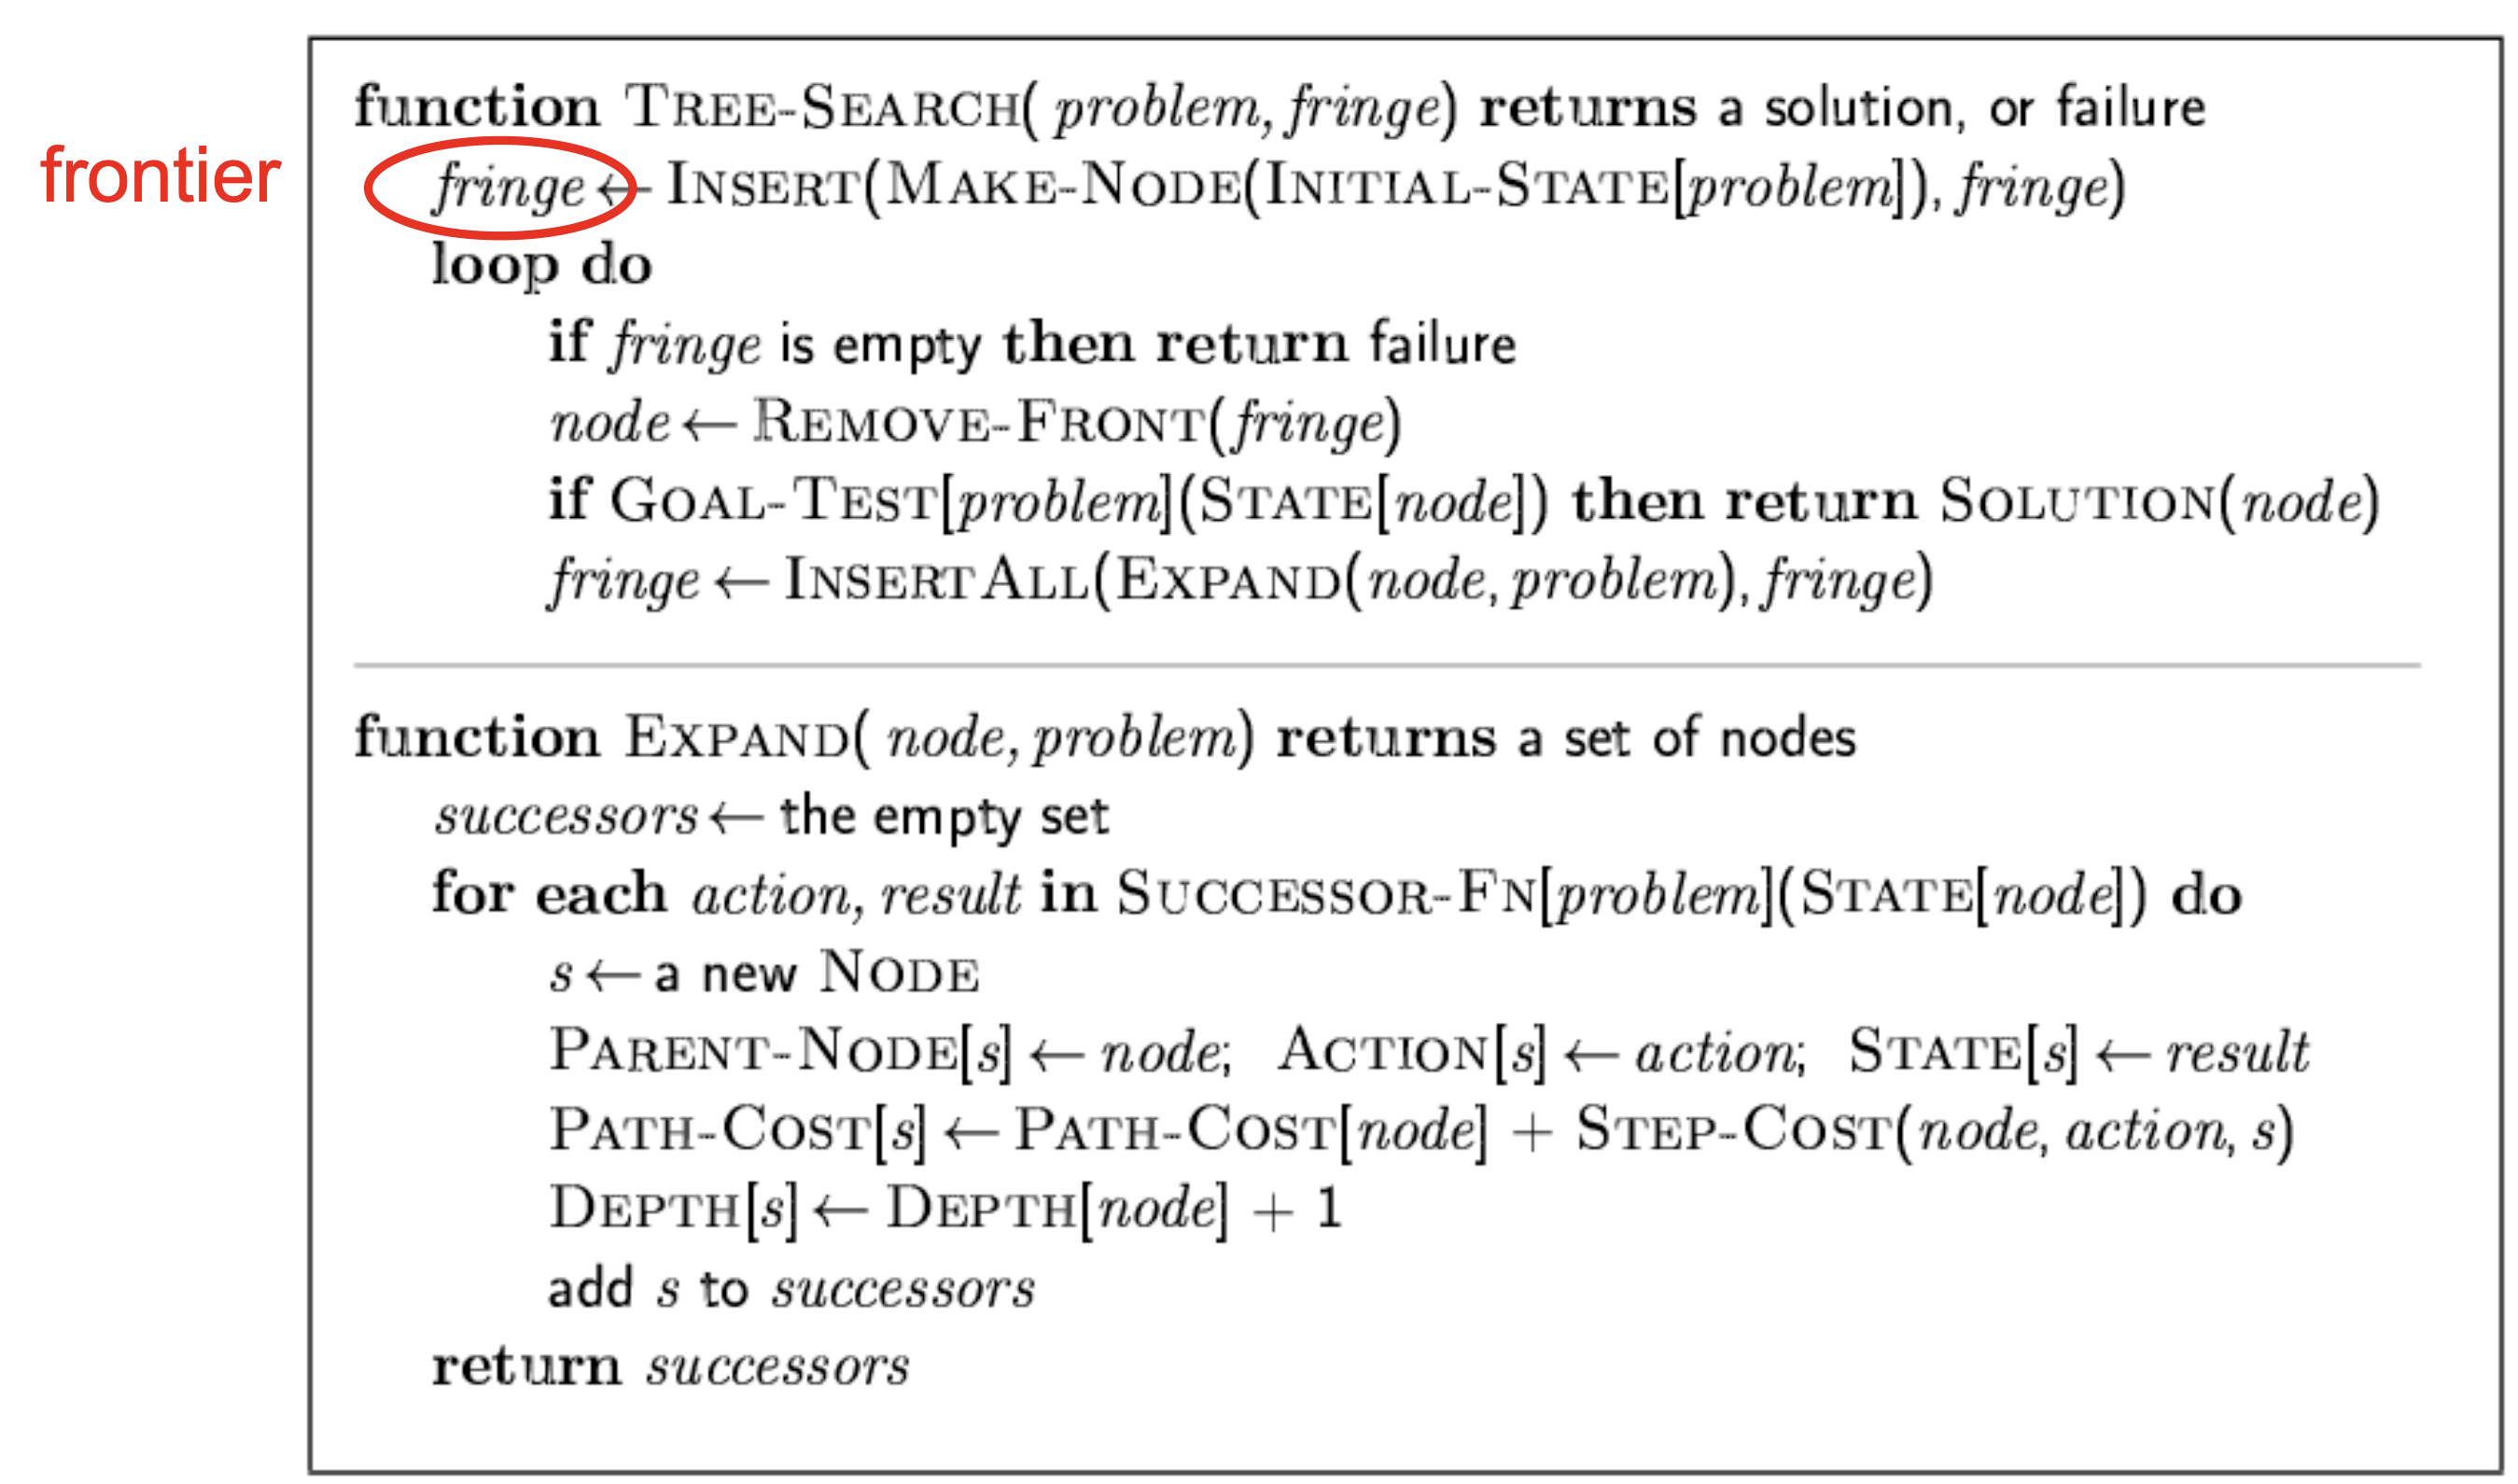
\includegraphics[width=0.85\columnwidth]{L2/tree-search} 
      \end{center}
      \begin{itemize}[leftmargin=*]
        \item May revisit nodes
        \item Checks for goal state \textbf{after} traversing to the node
      \end{itemize}
    \subsection*{Graph search} \noindent
      \vspace{-0.5cm}
      \begin{center}
        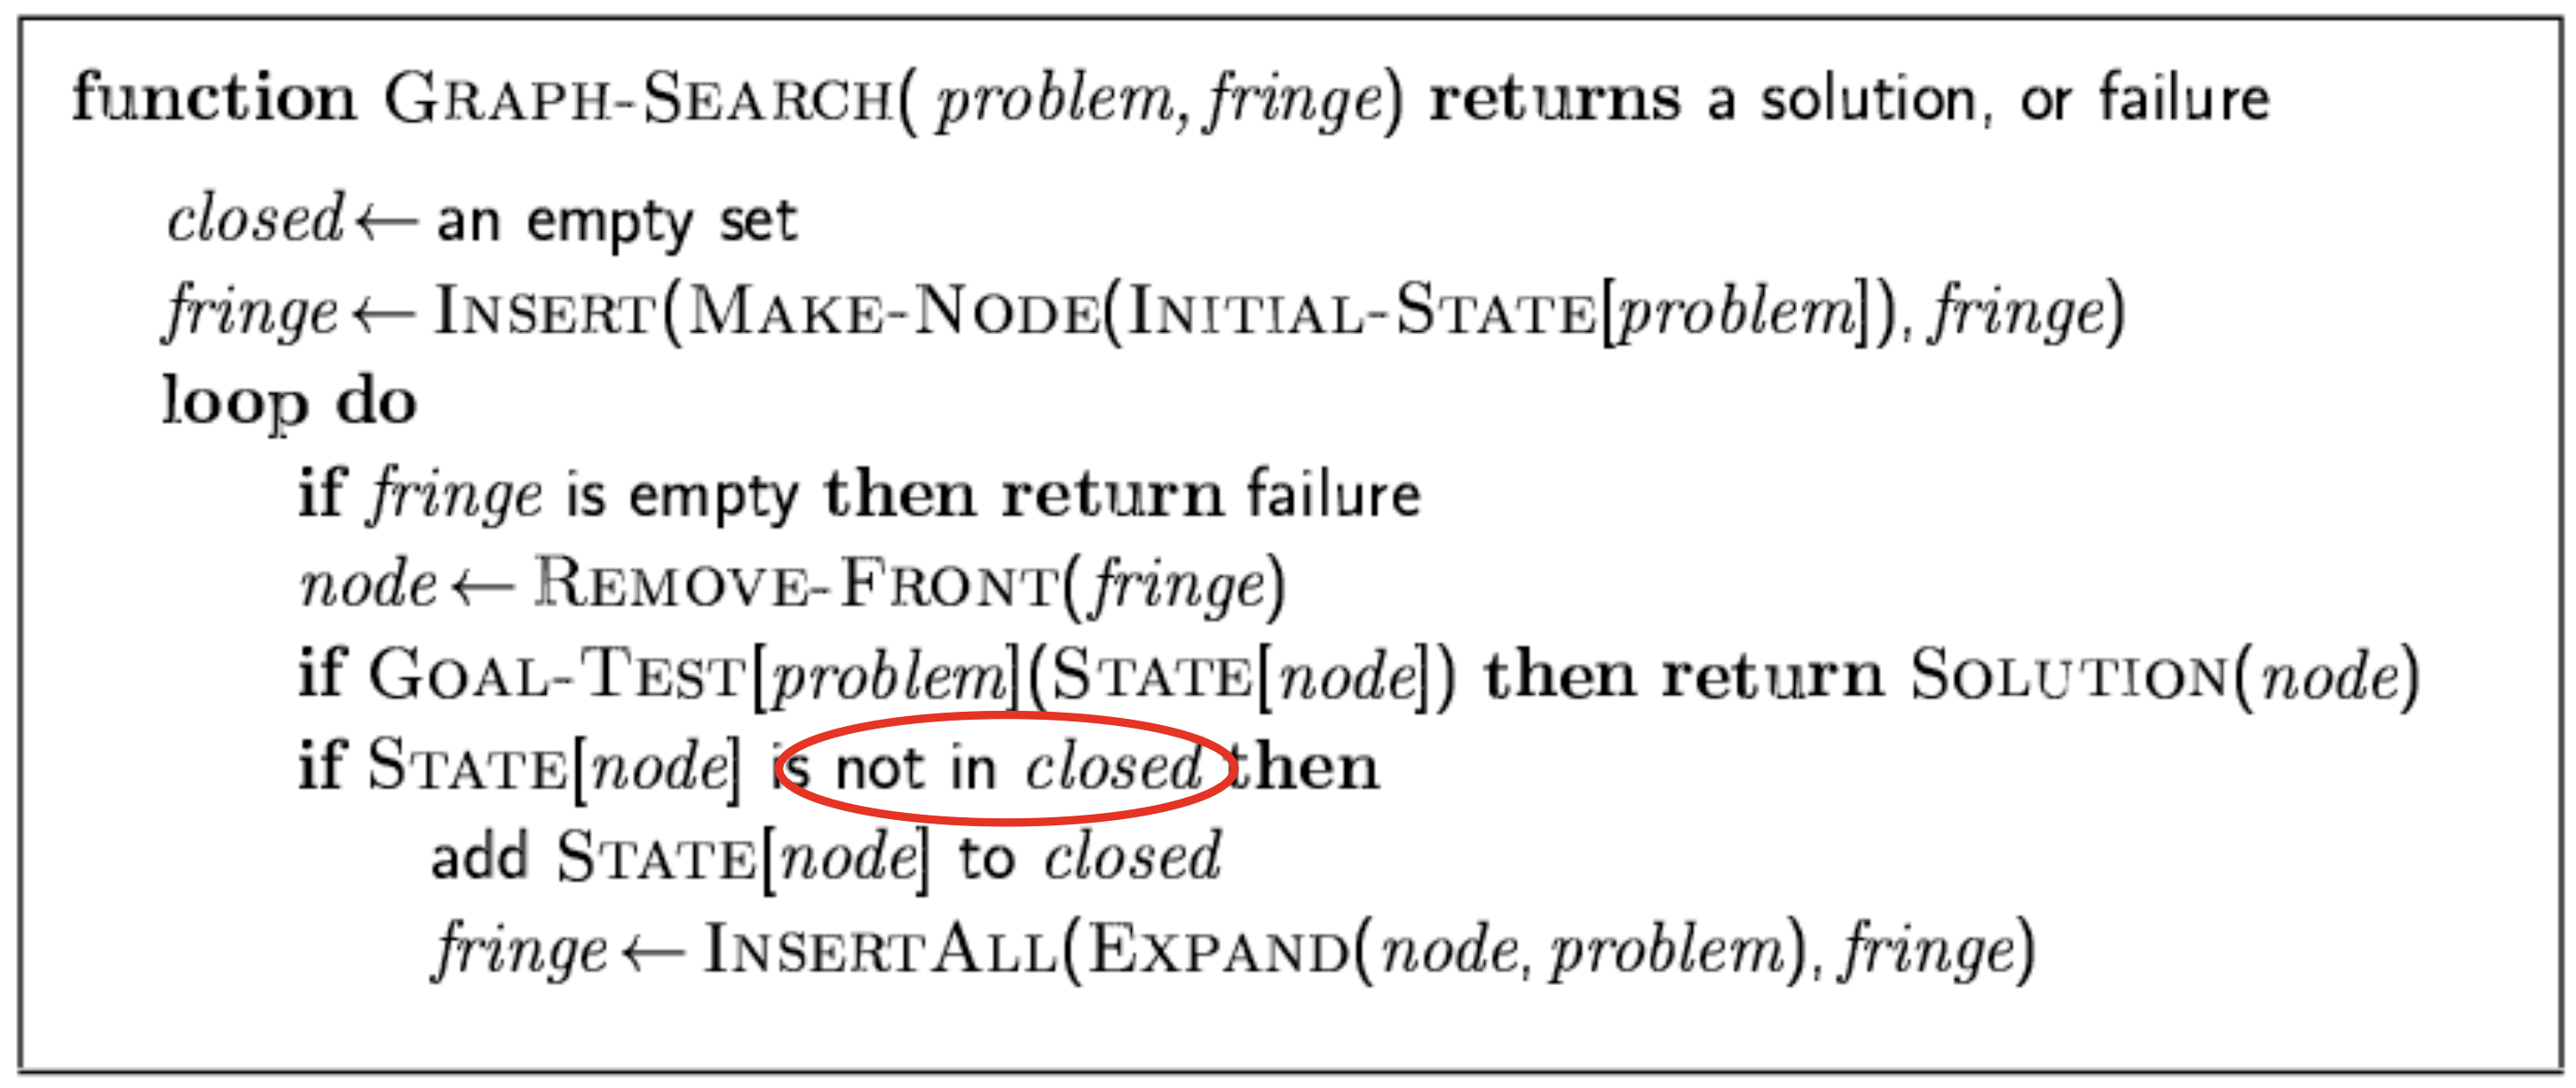
\includegraphics[width=0.85\columnwidth]{L2/graph-search}
      \end{center}
      \begin{itemize}[leftmargin=*]
        \item Will not revisit nodes
        \item Checks for goal state \textbf{after} traversing to the node
      \end{itemize}
    \subsection*{Bidirectional search}
      \begin{itemize}[leftmargin=*]
        \item Simultaneously search from initial state and backward state, and terminate when the two searches meet
        \item $2 \times O(b^\frac{d}{2}) < O(b^d)$
      \end{itemize}
      \paragraph{Implementation issues}
        \begin{itemize}[leftmargin=*]
          \item Succ(n) must be reversible/bidirectional
          \item Multiple goal states $\rightarrow$ Construct goal state containing superset of all goal states
          \item How to check if a node appears in the other search tree
          \item Can use different search strategies for each half
        \end{itemize}
  \section*{Informed Search}
    \subsection*{Best-first search}
      \begin{itemize}[leftmargin=*]
        \item Use an evaluation function $f(n)$ for each node, estimates desirability
        \item Expand most desirable unexpanded node
        \item e.g. Greedy best-first search, $A^*$ search
      \end{itemize}
      \paragraph{Greedy best-first search}
        \begin{itemize}[leftmargin=*]
          \item Expands node that appears closest to goal
          \item Can get stuck in loops
          \item Same as $A^*$ with $g(n) = 0$
        \end{itemize}
      \paragraph{$A^*$ search}
        \begin{itemize}[leftmargin=*]
          \item Avoid expanding expensive paths
          \item Evaluation function
            \[ f(n) = g(n) + h(n) \]
            \begin{align*}
              g(n) &= \text{cost so far to reach $n$} \\
              h(n) &= \text{estimated cost from $n$ to goal} \\
              f(n) &= \parbox{5cm}{estimated total cost of path, through $n$, to goal}
            \end{align*}
          \item Can be thought of as a variant for uniform-cost search, where cost is $f = g+h$
        \end{itemize}
    \subsection*{Admissible heuristics}
      \begin{itemize}[leftmargin=*]
        \item Heuristic $h$ is admissible if it never over-estimates the cost to reach the goal
        \item If $h(n)$ is admissible, then $A^*$ using tree search is optimal
      \end{itemize}
      \paragraph{Dominance} For admissible heuristic functions $h_1$ and $h_2$,
        \[ \forall n \; h_2(n) \geq h_1(n) \Rightarrow h_2 \text{ dominates } h_1 \]
        and $h_2$ is typically better for search.
      \paragraph{Inventing admissible heuristics}
        \begin{itemize}[leftmargin=*]
          \item A problem with fewer restrictions on the actions is called a \textbf{relaxed problem}
          \item Cost of an optimal solution to relaxed problem is an admissible heuristic for the original problem
          \item Non-admissible heuristics may be helpful for pruning, but lose optimality
        \end{itemize}
      \paragraph{Sample heuristics}
        \begin{itemize}[leftmargin=*]
          \item Manhattan distance (can only move horizontally/vertically)
          \item Number of pieces on the board
        \end{itemize}
    \subsection*{Consistent heuristics} \noindent
      \begin{minipage}{.65 \columnwidth}
        \begin{itemize}[leftmargin=*]
          \item A heuristic $h$ is consistent if for every node $n$ and successor $n'$ generated by action $a$,
            \[ h(n) \leq c(n, a, n') + h(n') \]
          \item Consistent $h \Rightarrow f(n)$ is non-decreasing along any path
          \item Consistent $h \Rightarrow h$ is admissible
          \item Consistent $h \Rightarrow A^*$ using graph search is optimal
        \end{itemize}
      \end{minipage}
      \hfill
      \begin{minipage}{.35 \columnwidth}
        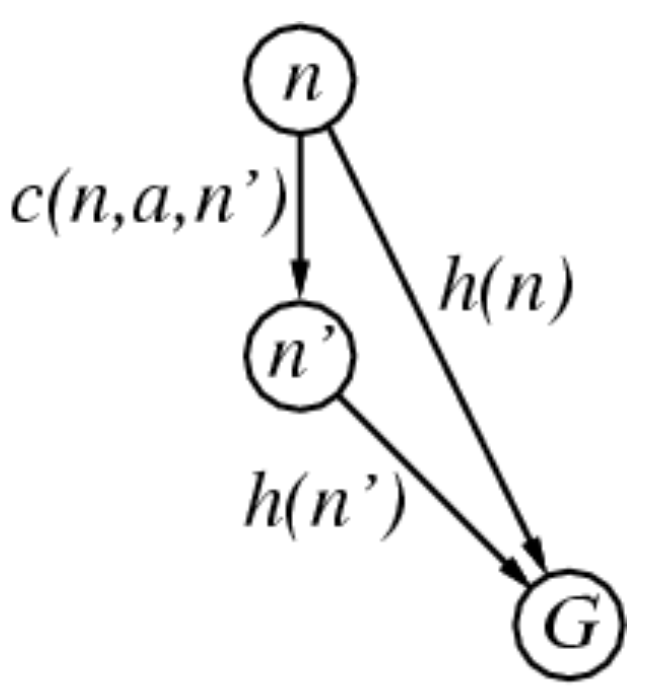
\includegraphics[width=\textwidth]{L3/consistent-heuristic}
      \end{minipage}
    \subsection*{Memory-bounded heuristic search}
      \paragraph{IDA$^*$} Use $f=g+h$ instead of depth for IDS cutoff
      \paragraph{Recursive best-first search}
        \begin{itemize}[leftmargin=*]
          \item Remember the 2nd best $f$-cost for all ancestors of node
          \item Expand from the best $f$-cost
          \item Once the $f$-cost in the current search exceeds any 2nd best $f$-cost among ancestors, continue from that instead
        \end{itemize}
      \paragraph{Criticism} $A^*$ and RBFS use linear space, which underutilizes available memory
      \paragraph{Simplified MA$^*$}
        \begin{itemize}[leftmargin=*]
          \item Run $A^*$ until memory full. When memory full,
            \begin{itemize}[leftmargin=*]
              \item Drop node with worst $f$-value
              \item Record on sub-tree
              \item If all better paths explored, regenerate this path
            \end{itemize}
        \end{itemize}
      \paragraph{Evaluating a heuristic}
        \begin{itemize}[leftmargin=*]
          \item Effective branching factor. With $N$ nodes generated, and solution depth $d$, compute $b^*$:
            \[ N+1 = 1 + b^* + (b^*)^2 + \cdots + (b^*)^d \]
            As $b^*$ gets closer to 1, the better the heuristic.
          \item Effective depth $d-k$, in $O(b^{d-k})$ vs $O(b^d)$
            As $k$ increases, the better the heuristic.
        \end{itemize}
    \subsection*{Local search}
      \begin{itemize}[leftmargin=*]
        \item Used when path to goal state is irrelevant; goal state is solution
        \item e.g. finding a configuration satisfying some contraints
      \end{itemize}
      \paragraph{Hill climbing}
        \begin{itemize}[leftmargin=*]
          \item Define objective function for each node
          \item Define actions/successor functions
          \item Given a starting node, recurse into highest-valued successor
          \item If the node has a higher value than successors, then return it. It is a local maximum, but may not be a global maximum
        \end{itemize}
        \vspace{-0.3cm}
        \begin{center}
          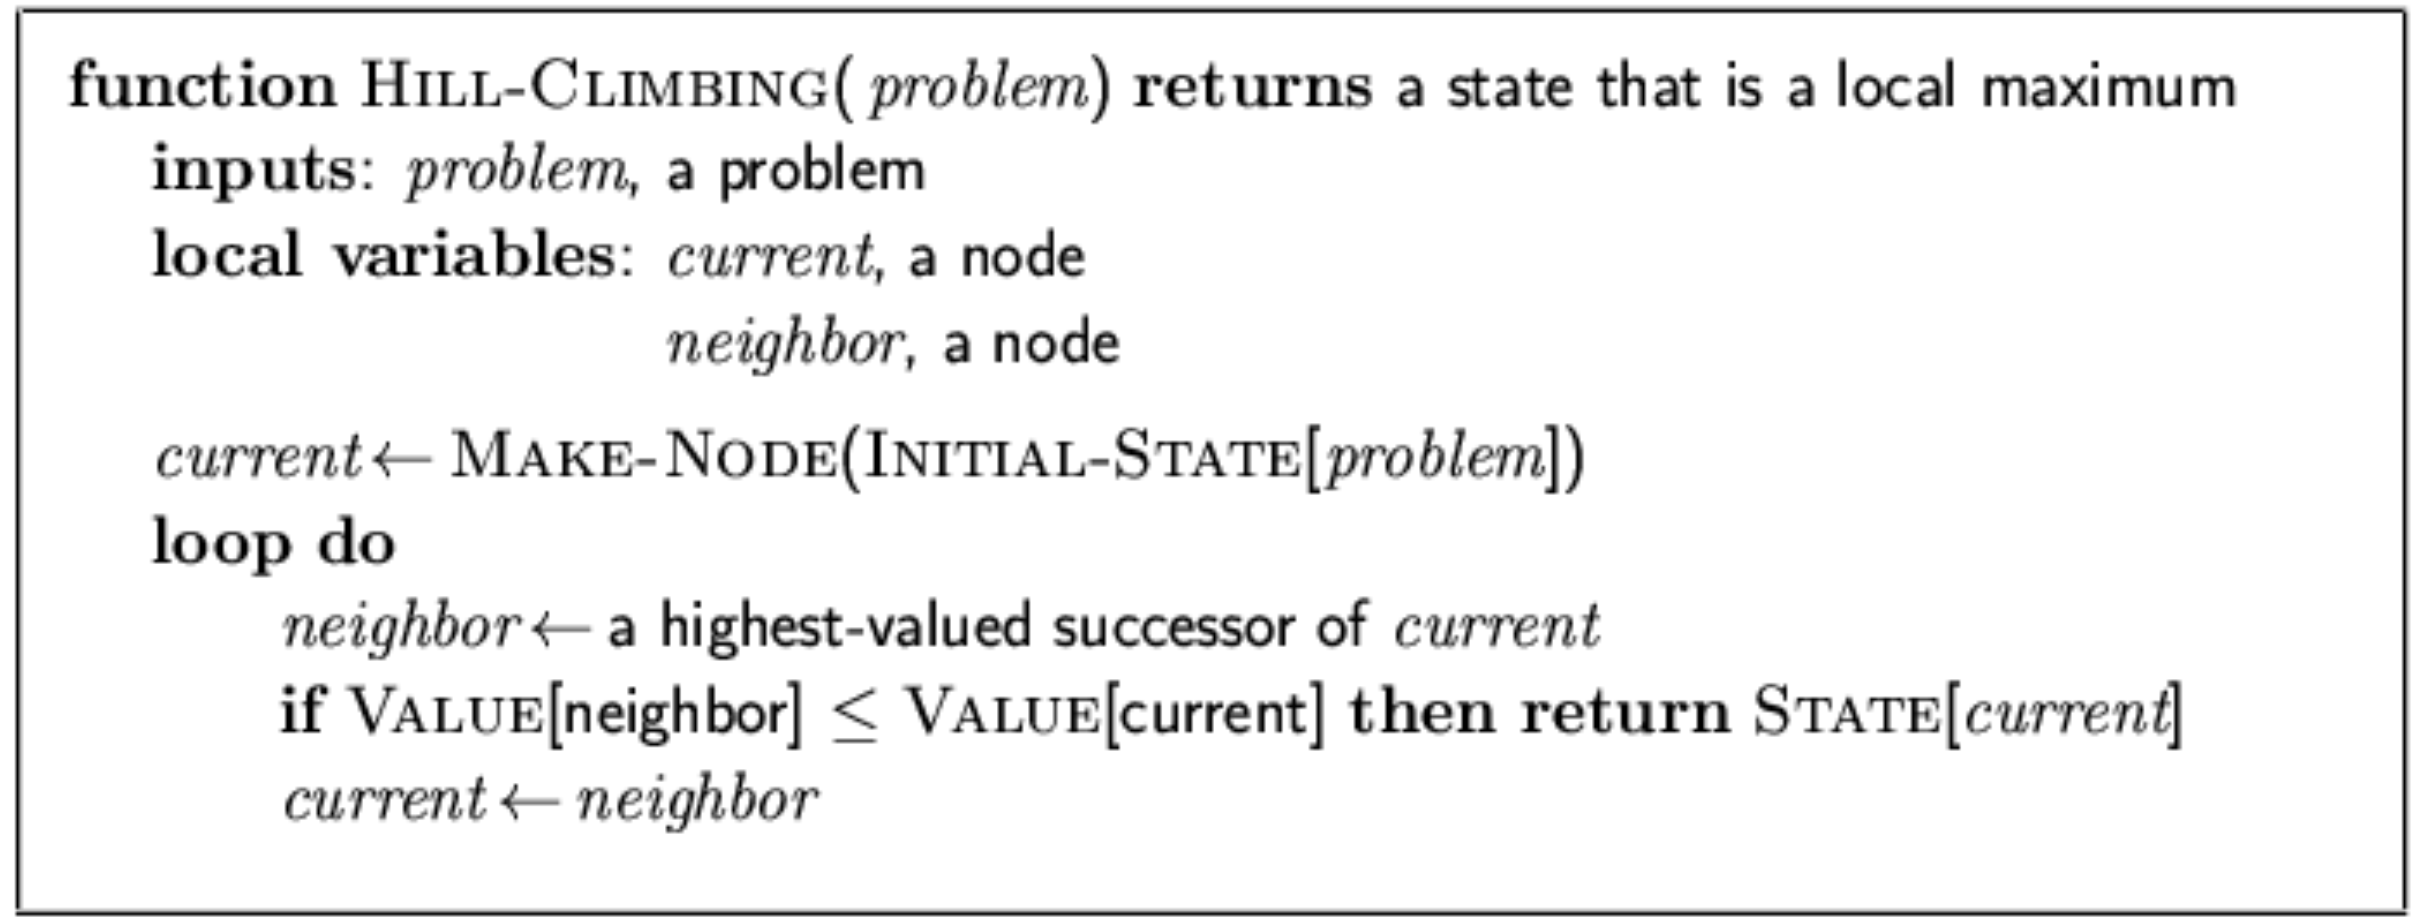
\includegraphics[width=0.85\columnwidth]{L3/hill-climbing}
        \end{center}
      \paragraph{Simulated annealing}
        \begin{itemize}[leftmargin=*]
          \item Randomly pick successor/action
          \item If successor has higher value, recurse. Otherwise recurse with a probability that exponentially decreases.
          \item Escapes local maxima by allowing bad moves occasionally
          \item If $T$ decreases slowly enough, then it finds a global optimum with probability approaching 1
        \end{itemize}
        \begin{center}
          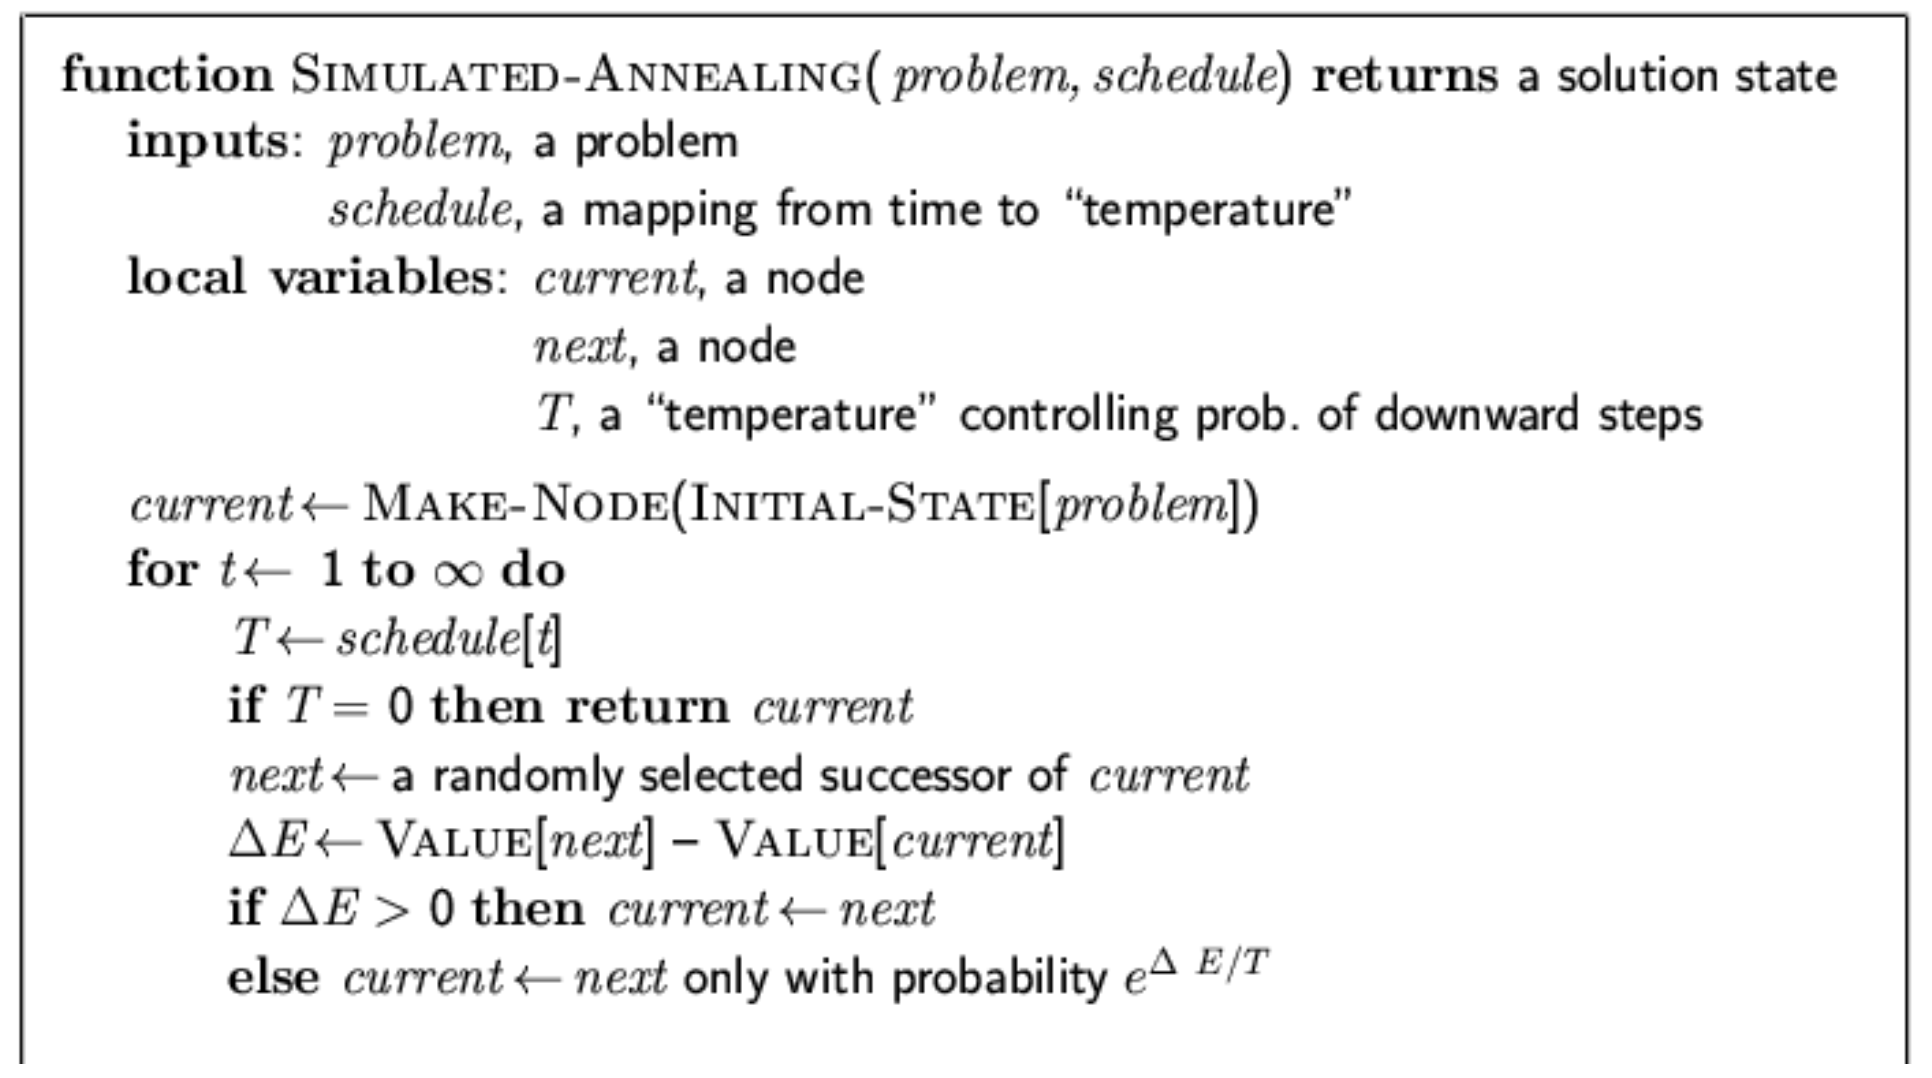
\includegraphics[width=0.95\columnwidth]{L3/simulated-annealing}
        \end{center}
      \paragraph{Beam search}
        \begin{itemize}[leftmargin=*]
          \item Perform $k$ hill-climbing searches in parallel
          \item Like BFS, but only take best $k$ nodes in each level
          \item Local beam search: the $k$ threads share info
          \item Stochastic beam search: $k$ independent threads
        \end{itemize}
      \paragraph{Genetic algorithms}
        \begin{itemize}[leftmargin=*]
          \item Start with $k$ randomly generated states
          \item States represented as a string over finite alphabet (often as a string of 0s and 1s)
          \item Evaluation (fitness) function has higher values for better states
          \item Generate successor state by combining two parent states via selection, crossover, mutation
        \end{itemize}
        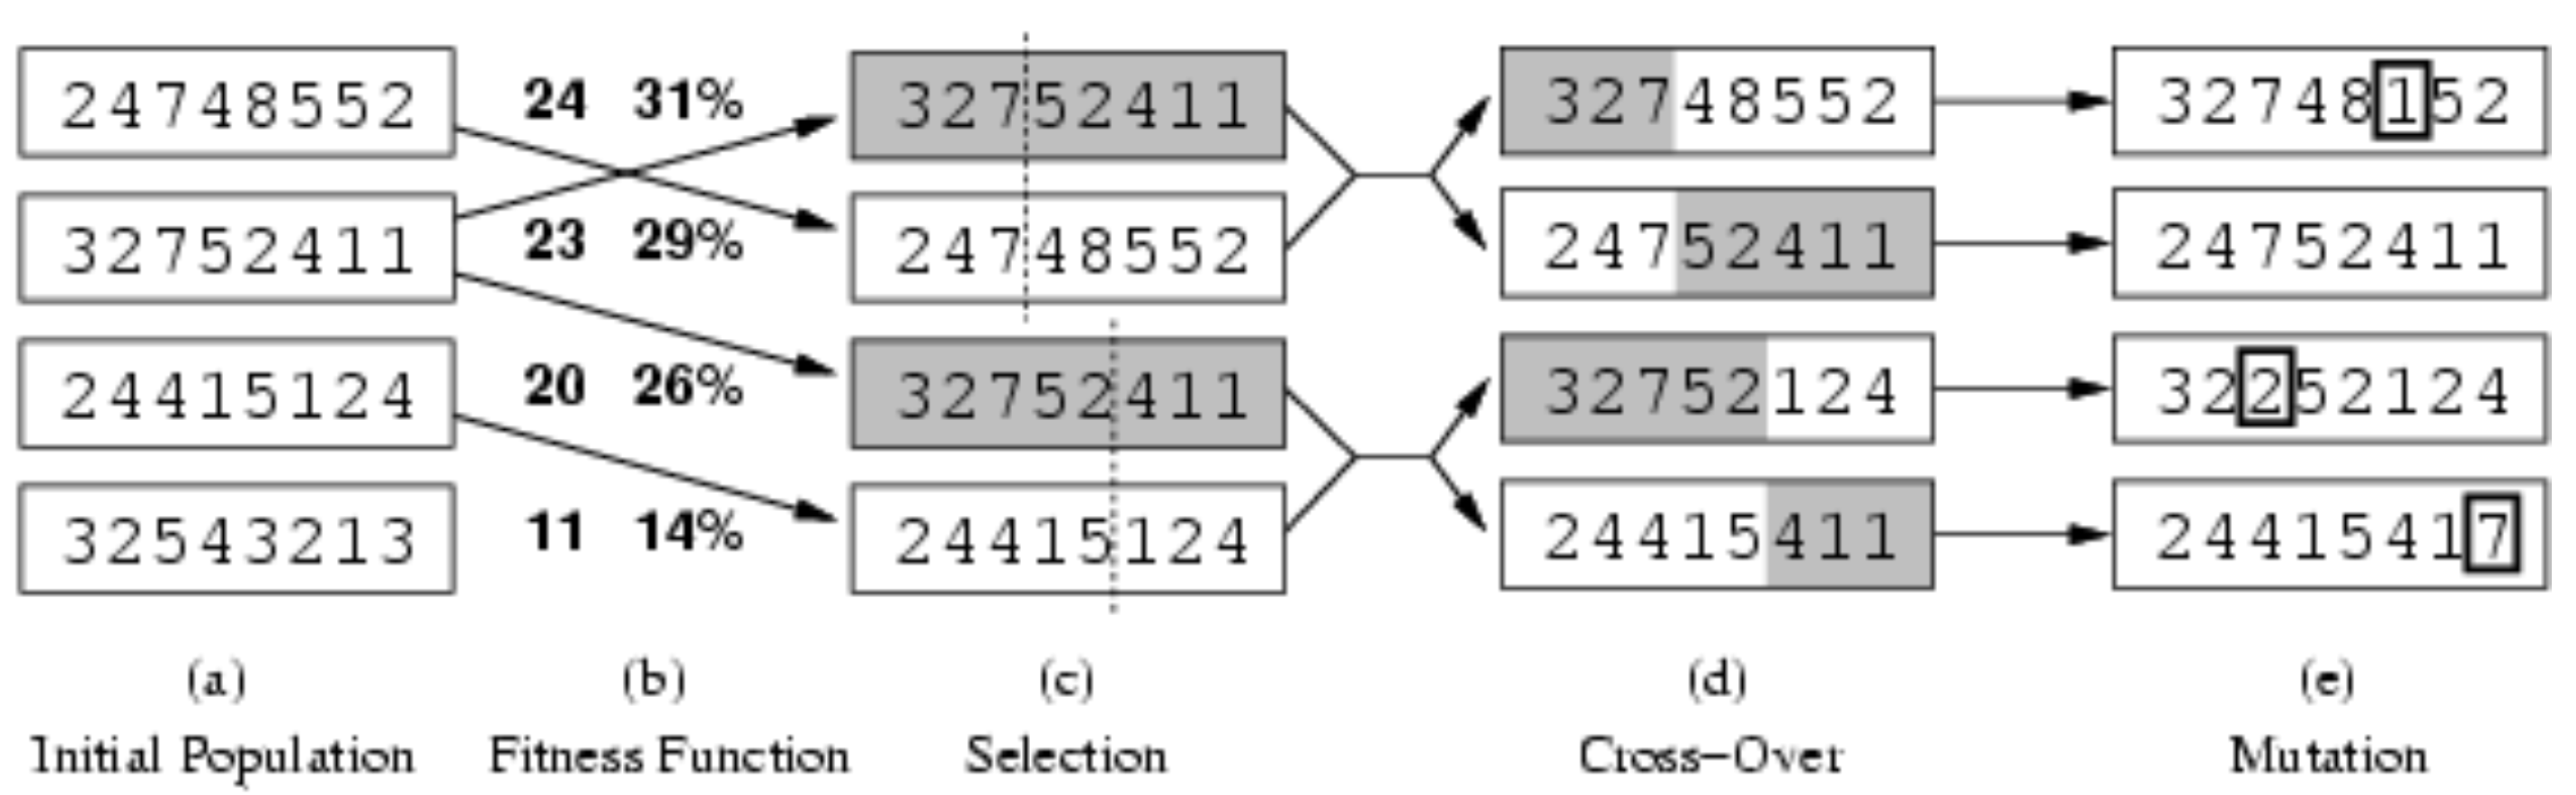
\includegraphics[width=\columnwidth]{L3/genetic}
\section*{Adversarial Search}
  \subsection*{Minimax}
    \begin{itemize}[leftmargin=*]
      \item Perfect play for deterministic games
      \item Choose move to position with highest minimax value
      \item Recursive algorithm (like DFS)
      \item Minimax algorithm is not optimal against non-optimal MIN player. MAX could have made high risk high reward moves if MAX knows that MIN was non-optimal, but MAX assumed that MIN was optimal and took a safer move, which is not optimal.
    \end{itemize}
    \begin{center}
      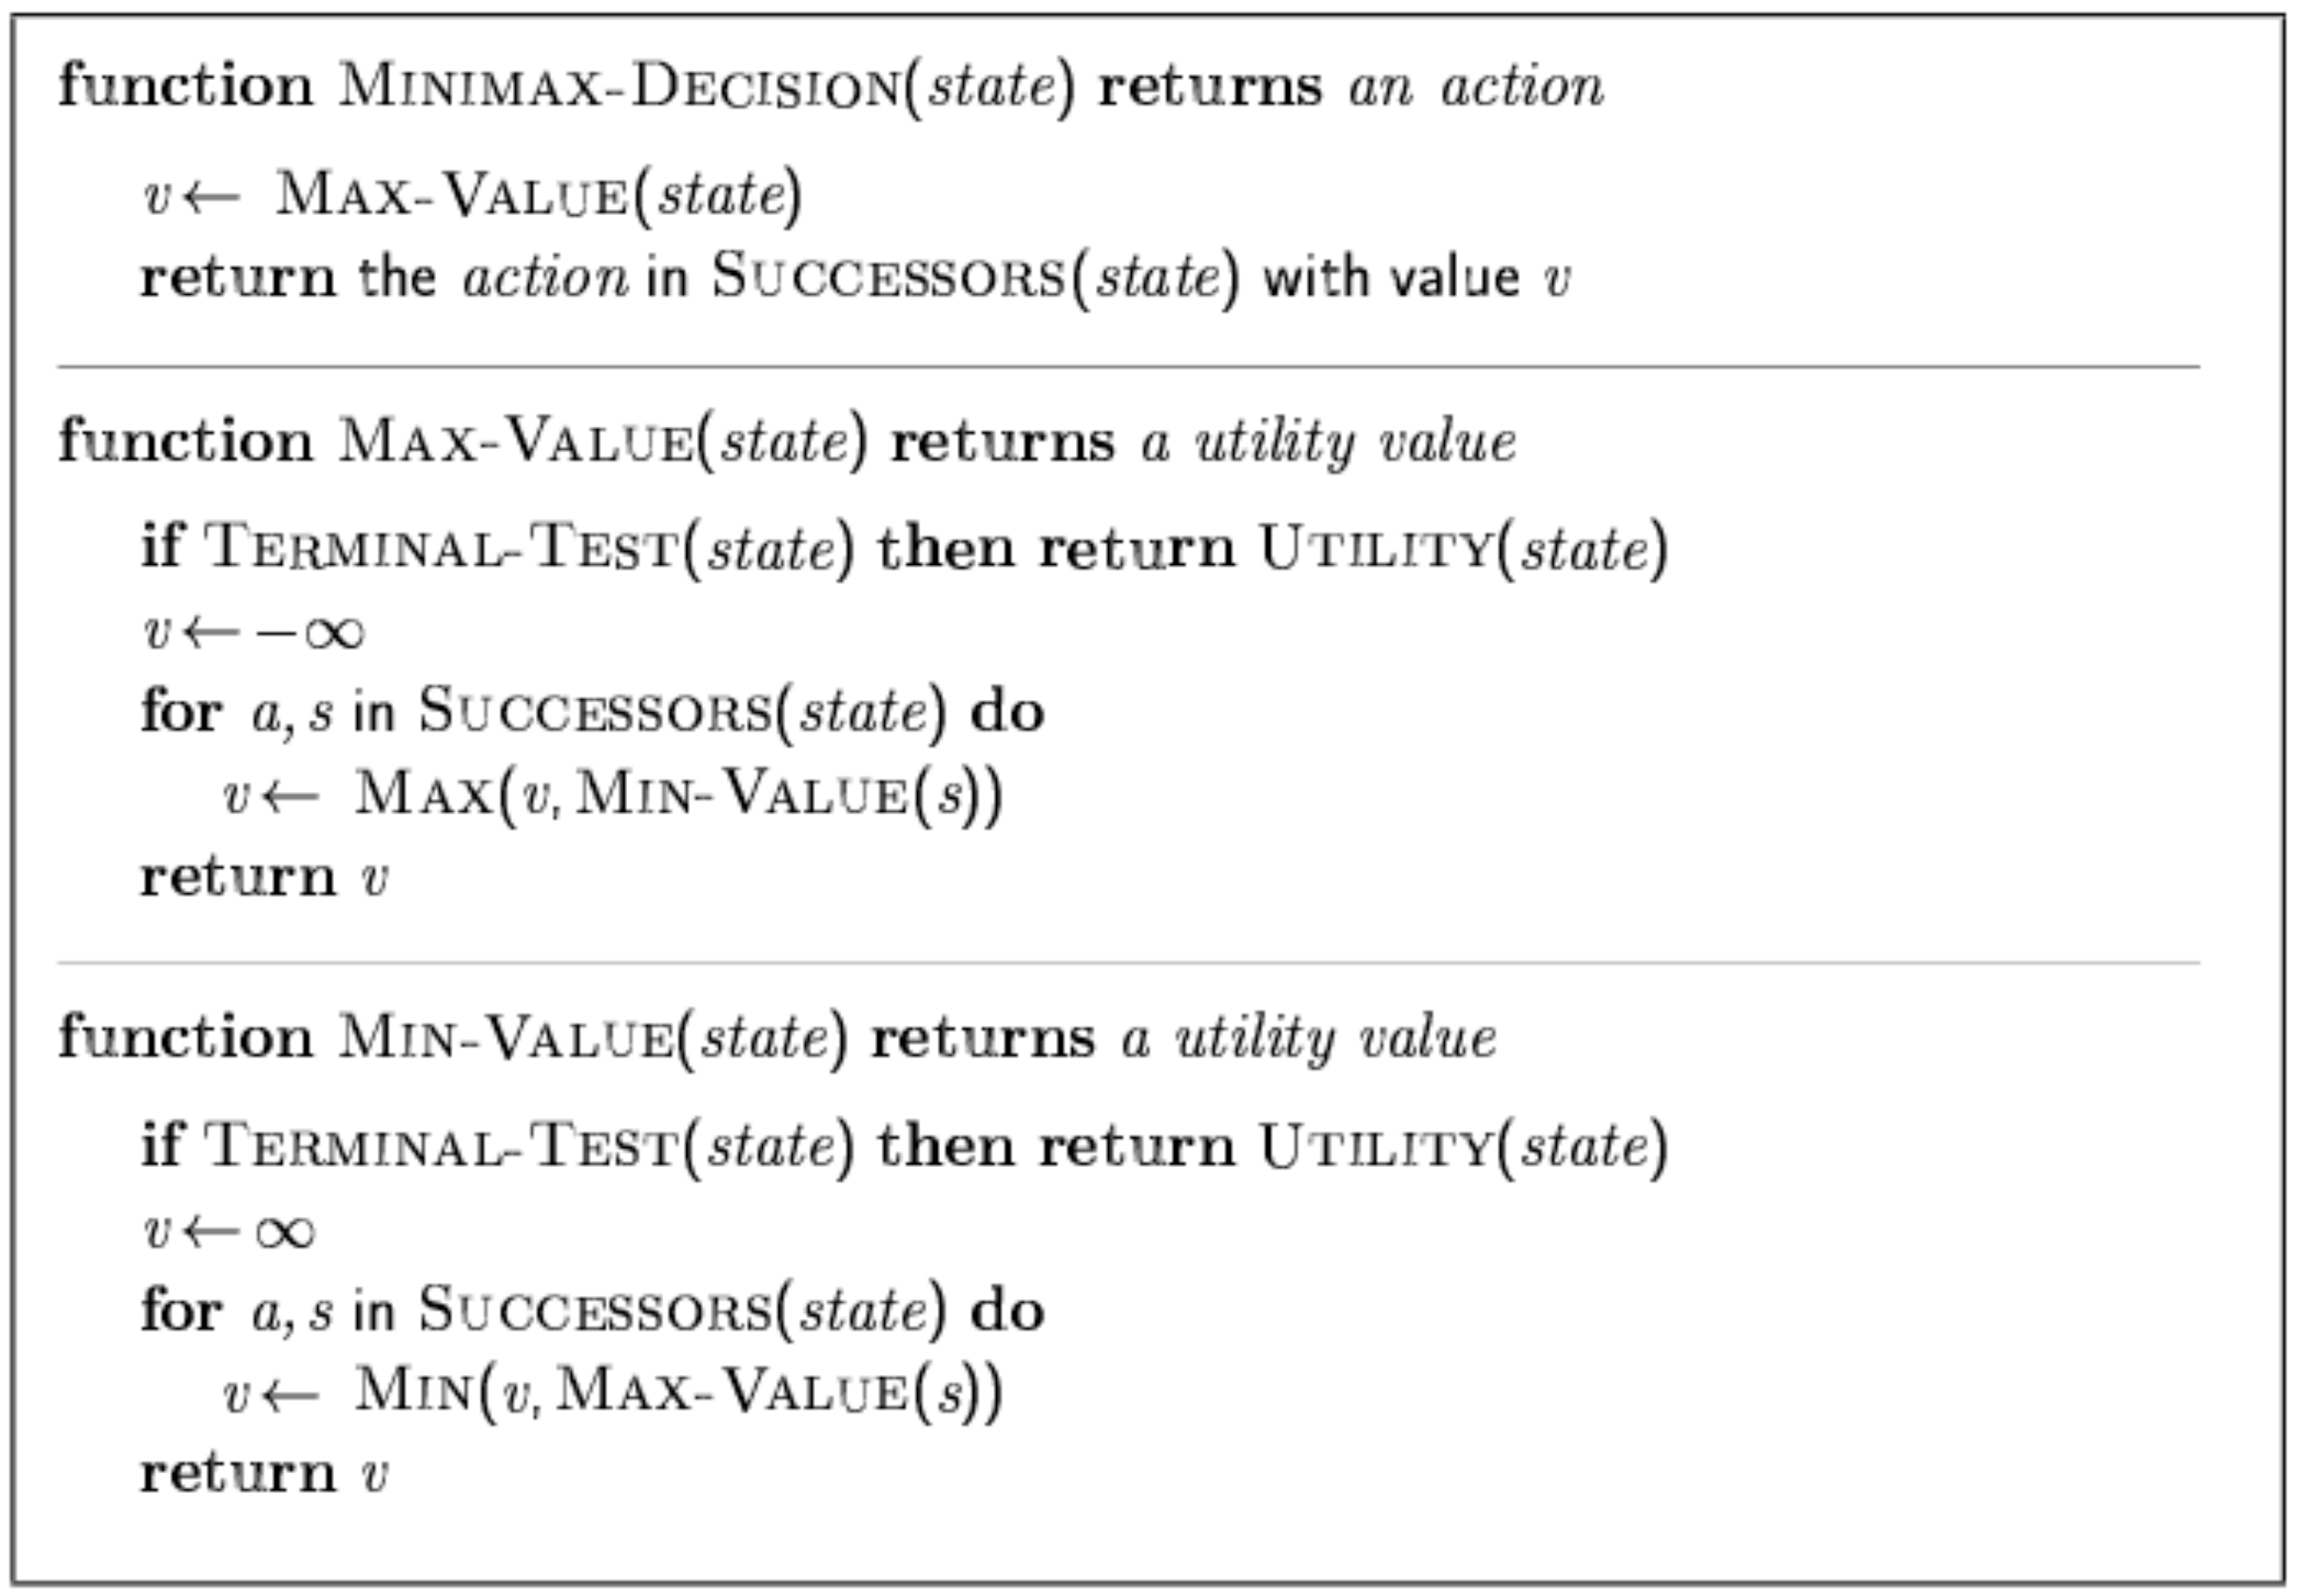
\includegraphics[width=0.95\columnwidth]{L4/minimax}
    \end{center}
  \subsection*{\ab pruning}
    \begin{itemize}[leftmargin=*]
      \item Skip (prune) less-optimal paths that will not be used
      \item At MIN node, stop if sibling has guaranteed higher value
      \item At MAX node, stop if sibling has guaranteed lower value
    \end{itemize}
    \begin{center}
      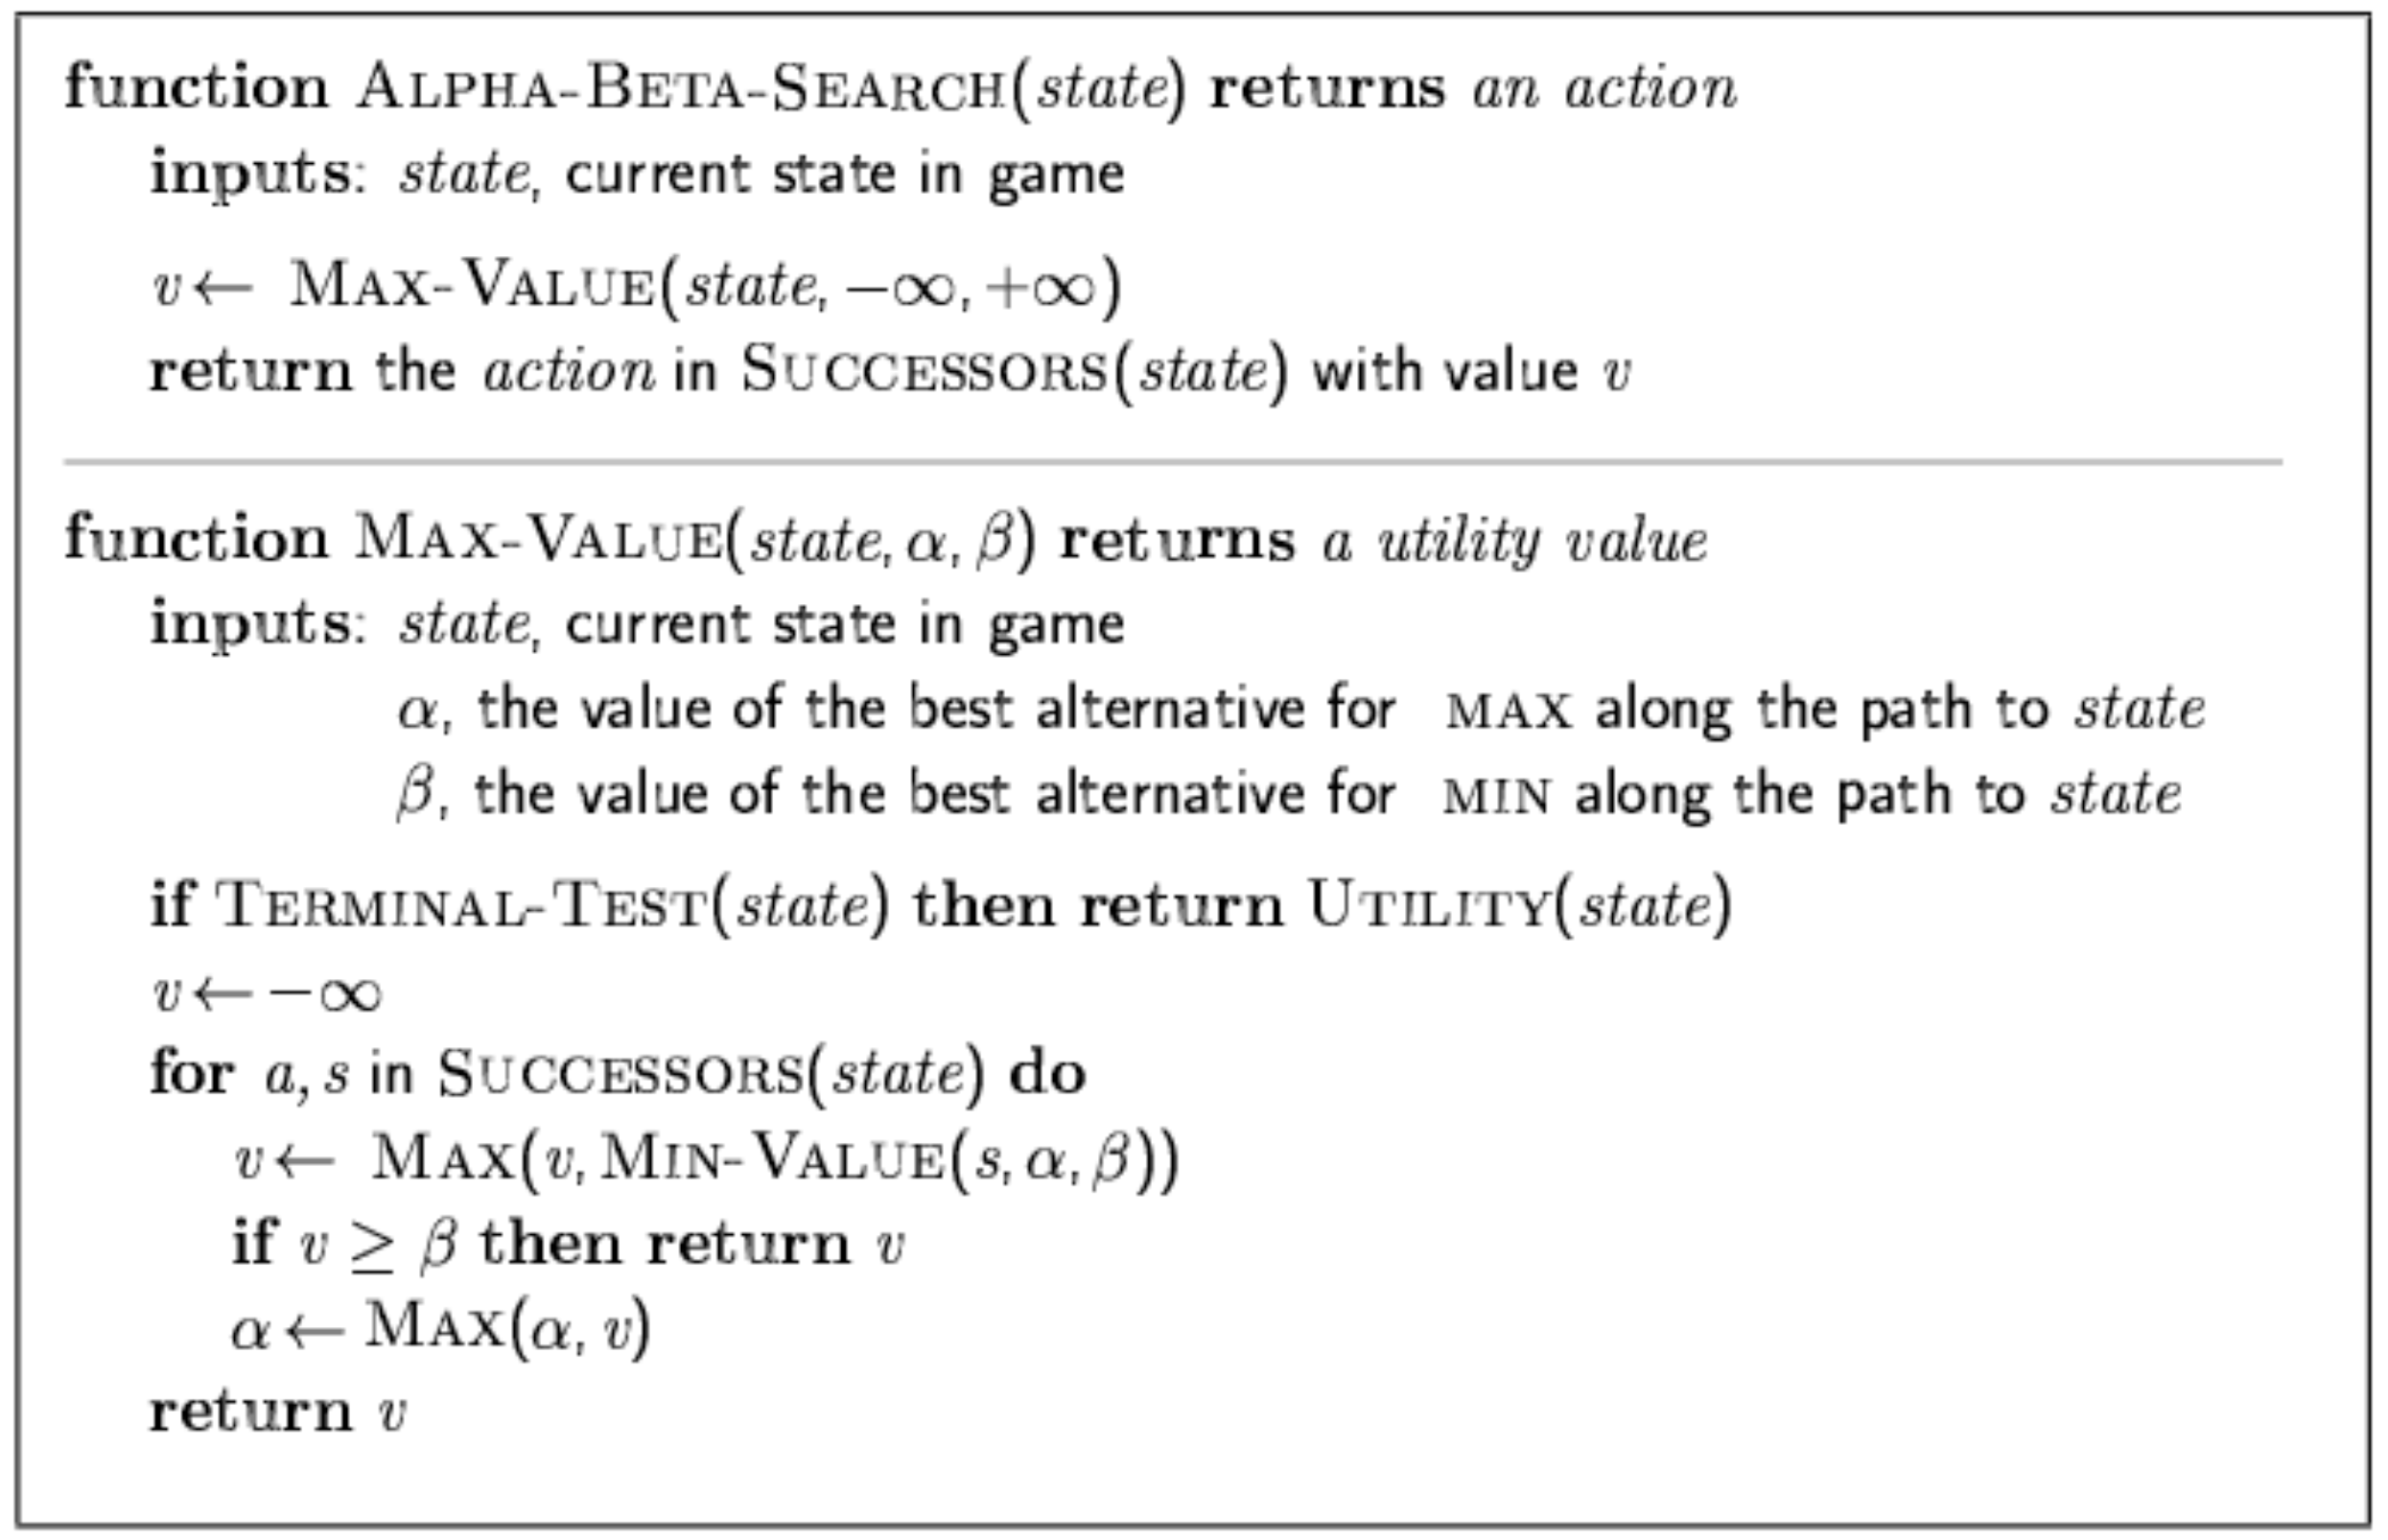
\includegraphics[width=\columnwidth]{L4/alpha-beta}
    \end{center}
    \paragraph{Properties}
      \begin{itemize}[leftmargin=*]
        \item Pruning should not affect final result
        \item Best case time complexity is $O(b^{m/2})$
      \end{itemize}
  \subsection*{Resource limits} \noindent
    Search space in games is typically large
    \begin{itemize}[leftmargin=*]
      \item Set depth limit to terminate early
      \item Use evaluation function to estimate desirability of position
      \item Transpositions: cache previously seen states, as different permuations of moves can lead to the same state
      \item Pre-compute opening/closing moves
    \end{itemize}
  \subsection*{Minimax Cutoff}
    \begin{itemize}[leftmargin=*]
      \item
        \begin{hlist}
          \item \textit{Terminal?} replaced by \textit{Cutoff?}
          \item \textit{Utility} replaced by \textit{Eval}
        \end{hlist}
      \item Sets a limit to the search depth
      \item $X$-ply: can recurse $X$ levels down
      \item In chess:
        \begin{hlist}
          \item 4-ply $\approx$ human novice
          \item 8-ply $\approx$ typical PC, human master
          \item 12-ply $\approx$ Deep Blue, Kasparov
        \end{hlist}
    \end{itemize}
  \subsection*{Evaluation functions}
    \begin{itemize}[leftmargin=*]
      \item Estimate the desirability of a certain state using the features
      \item e.g. Linear weighted sum in chess
        \[ Eval(s) = w_1 f_1(s) + w_2 f_2(s) + \cdots + w_n f_n(s) \]
        \begin{itemize}[leftmargin=*]
          \item Linear weighted sum assumes features are independent
          \item Might need to use non-linear/higher-order terms for dependent features
        \end{itemize}
    \end{itemize}
\section*{Machine learning}
  \paragraph{Definition}
    A computer program is said to learn from experience E with respect to some task T and some performance measure P, if its performance on T, as measured by P, improves with experience E. 
  \paragraph{Problem solving}
    \begin{enumerate}[leftmargin=*]
      \item Know exact formula $\rightarrow$ Direct Coding
      \item No formula, but have solution to related problem $\rightarrow$ Search
      \item Expert system
      \item Machine learning
    \end{enumerate}
  \paragraph{Data collection}
    \begin{itemize}[leftmargin=*]
      \item Costly
      \item Inconsistent data could mean:
        \begin{hlist}
          \item Hidden variables
          \item Noise
          \item Error
          \item All
        \end{hlist}
      \item Visualize to understand data
      \item More features/dimensions $\rightarrow$ exponentially more data needed
    \end{itemize}
\end{multicols*}
\begin{multicols*}{3}
  \paragraph{ML pipeline}
    \begin{hlist2}
      \item Data collection
      \item Data extraction (Feature engineering)
      \item Data understanding (with Visualization)
      \item Data pre-processing
      \item Model choice/design
      \item Model training
      \item Model validation (Evaluation)
      \item Model understanding (Visualization/Explainability)
      \item Model deployment
    \end{hlist2}
  \paragraph{Usefulness}
    \begin{itemize}[leftmargin=*]
      \item Not possible to program all human knowledge, e.g. facial recognition
      \item Less to program if machine can learn
      \item Can discover new knowledge
    \end{itemize}
  \subsection*{Types of feedback}
    \paragraph{Supervised}
      \begin{itemize}[leftmargin=*]
        \item Each example has correct answer
        \item e.g. image of ``A'' and unicode value 0041
        \item \textbf{Regression}: Predict results within a continuous output, map input variables to some continuous function
        \item \textbf{Classification}: Predict results in a discrete output, map input variables into discrete categories
      \end{itemize}
    \paragraph{Unsupervised}
      \begin{hlist}
        \item No answers given
        \item e.g. are there patterns in the data?
      \end{hlist}
    \paragraph{Weakly supervised}
      \begin{hlist}
        \item Correct answer given, but not precise
        \item e.g. image contains face (but exact location is not specified)
      \end{hlist}
    \paragraph{Reinforcement} \mbox{} \\
      \begin{hlist}
        \item Occasional rewards/penalties given
        \item e.g. robot navigating a maze
      \end{hlist}
  \subsection*{Decision trees}
    \begin{itemize}[leftmargin=*]
      \item Expresses a function of the input attributes, that maps to a decision (e.g true/false)
      \item Internal nodes are questions/tests, while leaf nodes represent the decision given the state
      \item Many possible orderings, want a compact tree $\Rightarrow$ choose attribute with largest information gain
    \end{itemize}
    \paragraph{Lecture Training}
      \begin{itemize}[leftmargin=*]
        \item Can be used for multi-label classification, by having each label as a leaf in the tree
        \item Can be used for regression, as it splits the data into smaller subsets. These subsets then can be assigned the most common results in the case of a regression.
        \item Two decision trees may be logically equivalent, but have different internal structure (i.e. they are different)
        \item Can use binary, discrete, or binned/discretized continuous valued attributes, but not continuous valued attributes
      \end{itemize}
    \paragraph{Pruning}
      \begin{itemize}[leftmargin=*]
        \item To reduce number of decision nodes
        \item To combine leaf nodes, take the more common result among the examples
      \end{itemize}
    \paragraph{Entropy}
      \begin{itemize}[leftmargin=*]
        \item Measure ``impurity'' or ``randomness'' in data
        \item Defined as \( \displaystyle I(P(v_1), \cdots, P(v_n)) = - \sum_{i=1}^n P(v_i) \log_2 P(v_i) \)
        \item For training set with $p$ positive examples and $n$ negative examples,
          \begin{flalign*}
            & I\left(\frac{p}{p+n}, \frac{n}{p+n}\right) = & \\
            & - \left(\frac{p}{p+n} \log_2 \frac{p}{p+n} +
            \frac{n}{p+n} \log_2 \frac{n}{p+n} \right)
          \end{flalign*}
      \end{itemize}
    \paragraph{Information gain}
      \begin{itemize}[leftmargin=*]
        \item Entropy of this node minus entropy of children nodes
        \item $p$ and $n$ refer to the examples at the node, $p_i$ and $n_i$ refer to the examples remaining at a specific child node
      \end{itemize}
      \resizebox{\columnwidth}{!}{\(\begin{aligned}
        \textrm{remainder}(A) &= \sum_{i=1}^v \frac{p_i+n_i}{p+n} I\left(\frac{p_i}{p_i+n_i}, \frac{n_i}{p_i+n_i}\right) \\
        IG(A) &= I\left(\frac{p}{p+n}, \frac{n}{p+n}\right) - \textrm{remainder}(A)
    \end{aligned}\)}
\section*{Linear regression} \noindent
  $m$ is the number of training samples
  \subsection*{Error function}
    \begin{itemize}[leftmargin=*]
      \item Using an error function for loss implies some meaning to the distance between predicted and actual values
      \item In classification, this distance is between class labels, so it may not make sense to use error functions for loss
    \end{itemize}
    \paragraph{Mean squared error (MSE)}
      Used for convenience, because it is differentiable everywhere
      \[ J(w_0, w_1) = \frac{1}{2m} \sum_{i=1}^m (h_w(x^{(i)}) - y^{(i)})^2 \]
    \paragraph{Mean absolute error (MAE)}
      \begin{itemize}[leftmargin=*]
        \item Not differentiable everywhere
        \item Emphasizes the error less, may be better if there are relatively many outliers in dataset
      \end{itemize}
  \subsection*{Gradient descent}
    \begin{itemize}[leftmargin=*]
      \item Gives a local minimum
      \item In implementation, learning rate $\alpha$ often decreases with more iterations (idea behind learning rate scheduler)
        \begin{itemize}[leftmargin=*]
          \item Start big to reach optimal values faster
          \item Slow down to allow for gradual convergence
        \end{itemize}
    \end{itemize}
  \subsection*{Single-variable gradient descent}
    \begin{itemize}[leftmargin=*]
      \item Hypothesis $h$ takes in a vector, returning a scalar
        \[ h_w(x) = w_0 + w_1x \]
      \item Cost function \[ J(w_0, w_1) = \frac{1}{2m} \sum_{i=1}^m (h_w(x^{(i)}) - y^{(i)})^2 \]
      \item Goal: Pick $w_0, w_1$ to minimize $J(w_0, w_1)$
    \end{itemize}
    \paragraph{Updating weights}
      \begin{itemize}[leftmargin=*]
        \item Update weights simultaneously using positive learning rate $\alpha$
      \end{itemize}
        \resizebox{\columnwidth}{!}{\(\begin{aligned}
          (w_0, w_1) := \left( w_0 - \alpha \frac{\partial J(w_0, w_1)}{\partial w_0}, \; w_1 - \alpha \frac{\partial J(w_0, w_1)}{\partial w_1} \right)
        \end{aligned}\)}
      \begin{itemize}[leftmargin=*]
        \item Partial derivatives:
      \end{itemize}
        \begin{align*}
          \frac{\partial J(w_0, w_1)}{w_0} &= \frac{1}{m} \sum_{i=1}^m (w_0 + w_1 x^{(i)} - y^{(i)})^2 \\
          \frac{\partial J(w_0, w_1)}{w_1} &= \frac{1}{m} \sum_{i=1}^m (w_0 + w_1 x^{(i)} - y^{(i)})^2 \cdot x^{(i)}
        \end{align*}
  \subsection*{Variants}
    \paragraph{Batch gradient descent} Consider all training examples at each iteration
    \paragraph{Stochastic gradient descent} Consider one data point at time
      \begin{itemize}[leftmargin=*]
        \item Faster
        \item More randomness - might escape local minima
      \end{itemize}
  \subsection*{Multivariable gradient descent}
    \begin{itemize}[leftmargin=*]
      \item Hypothesis $h$ takes in a vector, returning a scalar
        \[ h_w(x) = w_0 + w_1x_1 + w_2x_2 + \cdots + w_nx_n \]
        or
        \[ h_w(x) = w^Tx \]
    \end{itemize}
      where $w^T = \mat{w_0 w_1 \cdots, w_n}$ and $x^T = \mat{x_0 x_1 \cdots, x_n} = \mat{1 x_1 \cdots, x_n}$. \\
      The 1 introduced for the bias may be treated as another variable $x_0$.
    \begin{itemize}[leftmargin=*]
      \item Cost function
        \[ J(w) = \frac{1}{2m} \sum_{i=1}^m (h_w(x^{(i)}) - y^{(i)})^2 \]
      \item Goal: Pick $w$ to minimize $J(w)$
    \end{itemize}
    \paragraph{Updating weights}
      \begin{align*}
        w_j &:= w_j - \alpha \frac{\partial J(w)}{\partial w_j} \quad \text{simultaneously for all $w_j$} \\
            &= w_j - \alpha \frac{1}{m} \sum_{i=1}^m (h_w(x^{(i)}) - y^{(i)}) \cdot x_j^{(i)}
      \end{align*}
  \subsection*{Feature scaling}
    \begin{itemize}[leftmargin=*]
      \item Gradient descent may not work well if features have signficantly different scales
      \item Perform mean normalization \( x_i := \dfrac{x_i - \mu_i}{\sigma_i} \)
      \item Useful in polynomial regression, where features likely have significantly different scales
    \end{itemize}
  \subsection*{Polynomial regression}
    \begin{itemize}[leftmargin=*]
      \item Generate new features which are higher-order terms of the original ones
      \item With a dataset of $N$ points, the max degree polynomial one should use is $N-1$. This is the least degree required to fit to all $N$ points; any higher degree polynomial would be overfitting.
    \end{itemize}
  \subsection*{Normal equation} \noindent
    Define design matrix $X$ and output vector $Y$ as follows:
    \[ X = \mat{1 (x^{(1)})^T; 1 (x^{(2)})^T; \vdots, \vdots; 1 (x^{(n)})^T}, \quad Y = \mat{y^{(1)}; y^{(2)}; \vdots; y^{(m)}} \]
    where each row corresponds to a sample. Then
    \[ w = (X^T X)^{-1} X^T Y \]
    \paragraph{Properties}
      \begin{hlist}
        \item No need to choose $\alpha$
        \item No iterations
        \item $X^T X$ needs to be invertible
        \item Slow if $n$ is large - $O(n^3)$
      \end{hlist}
    \paragraph{What if $X^T X$ is not invertible}
      \begin{itemize}[leftmargin=*]
        \item Infinite solutions to the normal equation
        \item Possible reasons:
          \begin{itemize}[leftmargin=*]
            \item If $m < n$, i.e. \# training data $<$ number of features, $X^T X$ is always not invertible. More data is required to get a unique solution.
            \item Not all columns are linearly independent. Consider removing one feature that might be dependent on a linear combination of others
          \end{itemize}
      \end{itemize}
\end{multicols*}
\end{document}
